\documentclass[11pt]{article}
\usepackage{geometry}
\geometry{a4paper, top=3cm, bottom=3cm}
\usepackage[utf8]{inputenc}
\usepackage{ngerman}
\usepackage{xcolor}
\usepackage{graphicx}
\usepackage{hyperref}
\usepackage{float}
\usepackage{subfigure}

%%%%%%%%%%%%%%%%%%%%%%%%%%%%%%%%%%%%%%%%%%%%%%
%        Document settings and title         %
%%%%%%%%%%%%%%%%%%%%%%%%%%%%%%%%%%%%%%%%%%%%%%
% In German, new paragraphs are not indented
\setlength{\parindent}{0cm}

% Define new command for red color emphasis
\newcommand{\red}[1]{\textcolor{red}{#1}}

% Title section
\title{
  \vspace{2cm}
  \Huge System Design Projekt \\
  \LARGE Zwischenbericht WS 2019/2020
}
\author{ \Large \red{Roberto (\#112)}\\ }
\date{ 06. Januar 2020 }

%%%%%%%%%%%%%%%%%%%%%%%%%%%%%%%%%%%%%%%%%%%%%%
%            Document starts here            %
%%%%%%%%%%%%%%%%%%%%%%%%%%%%%%%%%%%%%%%%%%%%%%
\begin{document}
\maketitle  % Inserts the title into document

\section{Gruppenmitglieder}
\begin{itemize}
  \item Viktor Gange (4924109)
  \item Igor Erfordt (4913715)
  \item Anna Nachname (Matrikelnummer)
  \item Xinjing Nachname (Matrikelnummer)
\end{itemize}

\section{Durchführung}
Unsere Gruppe verwendet den EV3-Roboter. Programmiert haben wir mit Visual Studio Code mit der Sprache Python 3. Die Verbindung zum Roboter haben wir über einen Wlan-Stick und mit Hilfe von VS-Code realisiert. Dabei haben wir die Offiziellen Dokumentationen von EV3 benutzt\footnote{https://ev3dev-lang.readthedocs.io/projects/python-ev3dev/en/stable/sensors.html}. Unsere ursprüngliche Idee war es mit zwei Lichtsensoren auszukommen. Die Linienverfolgung mit zwei Sensoren stellte sich jedoch schwieriger als gedacht heraus. Ein Bild vom alten aussehen beim Meilenstein sieht man im Bild \ref{Figure:roberto_alt}. Also beschloßen wir unseren Roboter nach dem Meilenstein komplett umzubauen, diesmal mit drei Lichtsensoren. Das neue Aussehen des Roboters zum Stand von 06.01.2020 kann man auf den Bild \ref{Figure:bild2} und \ref{Figure:bild3} sehen.

\subsection{Linienverfolgung}
Es werden 3 Lichtsensoren verwendet, dabei ist der mittlere immer auf der schwarzen Linie, und die äußeren Sensoren außerhalb der Linie. Wenn also einer der äußeren Sensoren auf die Linie kommt korrigiert der Roboter die Ausrichtung.

\subsection{Schranke}
Wenn der mittlere Sensor auf Schwarz ist und der Abstand zur Wand vom Ultraschaltsensor mit weniger als 8cm gemessen wird dann bleibt der Roberto so lange stehen bis der Ultraschallsensor einen Wert größer als 8cm misst.

\subsection{Klotz wegschieben}
Ist noch nicht Implementiert.

\subsection{Tunnel}
Wir haben so programmiert, dass man den Lichtwert an einer Stelle ändern muss wenn sich die Lichtbedingungen ändern. Der Tunnellauf funktioniert auf der Testbahn.

\subsection{Steigung und Gefälle}
Wir haben einen dritten Motor eingebaut und werden Steigung und Gefälle demnächst testen.

\subsection{Umgang mit dem Ball}
Ist noch nicht implementiert.

\begin{figure}[H]
  \centering
  % Image with 70% of document width.
  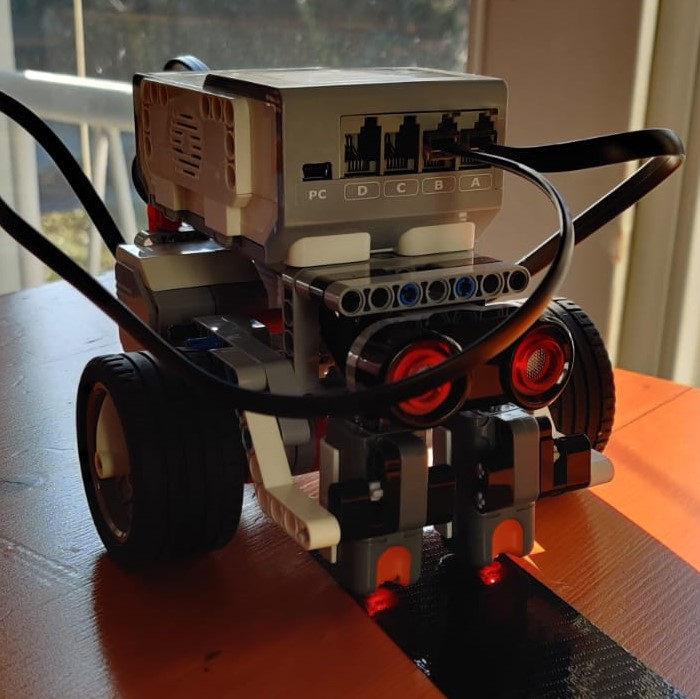
\includegraphics[width=0.7\textwidth]{roberto_alt.jpeg}
  \caption{Roberto beim Meilenstein}
  \label{Figure:roberto_alt}
\end{figure}

% Subfigure with multiple images
\begin{figure}[H]
  \centering
  \subfigure[Frontansicht]{
    \includegraphics[width=0.47\textwidth]{example-image.png}
    \label{Figure:Front}
  }
  \subfigure[Seitenansicht]{
    \includegraphics[width=0.47\textwidth]{example-image.png}
    \label{Figure:Side}
  }
  \caption{Bilder der Front- und Seitenansicht unseres NXT Roboters.}
  \label{Figure:RobotPics}  % Labels are used for referencing with \ref{}
\end{figure}

\section{Fehleranalyse}
Wir hatten am Anfang mit zwei Sensoren Probleme mit dem rechten Winkel(dabei sind beide Sensoren gleichzeitig auf weiß gewesen), dadurch mussten wir eine extra Funktion einbauen, die die Linie wieder gesucht hat. Das hat viel Zeit gekostet und war nicht zuverlässig, weshalb wir auch auf drei Lichtsensoren umgestiegen sind. Allgemein wenn wir Probleme mit Linienverfolgung hatten, haben wir versucht auf einem Blatt Papier das Problem nachzustellen um zu verstehen welcher Teil des Codes nicht optimal ist.

\section{Weiteres Vorgehen}
Als nächstes werden wir uns um die noch nicht Implementierten Funktionen widmen. Wenn das erledigt ist machen wir uns an die Optimierung der Zeit und Konsistenz.

\section{Arbeitsteilung}
Wir haben uns immer als volle Gruppe getroffen. Die Arbeiten an dem Code fanden also immer zusammen statt. Alle Gruppenteilnehmer haben sich an dem Code beteiligt.

\end{document}